\documentclass[serif,mathserif]{beamer}
\usepackage[portuguese]{babel}
\usepackage[utf8]{inputenc}
\usepackage{amsmath, amsfonts, epsfig, xspace}
\usepackage{algorithm,algorithmic}
\usepackage{pstricks,pst-node}
\usepackage{multimedia}
\usepackage[normal,tight,center]{subfigure}
\setlength{\subfigcapskip}{-.5em}
\usepackage{beamerthemesplit}
\usetheme{lankton-keynote}
\setbeamerfont{title}{size=\large}

\newcommand{\CcImageBy}[1]{%
  
\includegraphics[scale=#1]{creative_commons/cc_by_30.pdf}%
}
\newcommand{\CcImageSa}[1]{%
  
\includegraphics[scale=#1]{creative_commons/cc_sa_30.pdf}%
}
\newcommand{\CcGroupBySa}[2]{% zoom, gap
  \CcImageBy{#1}\hspace*{#2}\CcImageSa{#1}%
}
\newcommand{\CcLongnameBySa}{Attribution-ShareAlike}
\newcommand{\CcNote}[1]{% longname
  This work is licensed under the \textit{Creative Commons #1 3.0 License}.%
}

\author[Alessandro Palmeira]{Alessandro Palmeira}

\title[Software Livre e Ensino\hspace{2em}\insertframenumber/\inserttotalframenumber]{Software deve ter dono? Deve ser livre? Escolas devem usar software livre?}

\date{22 de Abril de 2015} %leave out for today's date to be insterted

\institute{MAC0470 - Desenvolvimento de Software Livre}


\begin{document}


\begin{frame}
  \titlepage
  \begin{center}
    \CcGroupBySa{0.83}{0.95ex}\\
    {\tiny\CcNote{\CcLongnameBySa}}
  \end{center}
\end{frame}



\section{Prólogo}  % add these to see outline in slides

\begin{frame}
  \frametitle{Prólogo}
  Por um instante, vamos pensar em toda a cultura gerada antes da Idade Moderna.\pause\\
  Tudo: Literatura, Pintura, Música, Arquitetura, Teatro, etc.\pause

  \vspace{5mm} %5mm vertical space
  Agora vamos pensar só em um pequeno subconjunto disso tudo...
\end{frame}

\begin{frame}
  Software\pause
  ... ou melhor, tudo aquilo que são instruções para resolver algum problema, desde a
  sua fome até a infinidade dos números primos.\pause\\
  Como fazer um pão, \pause como fazer um bolo, \pause como forjar uma espada, \pause como construir uma casa, \pause
  como tecer uma roupa, \pause como curtir couro, \pause como construir um arco, \pause como atirar com um arco, \pause
  como construir uma flauta, \pause como tocar uma flauta, \pause como cozinhar o barro e fazer potes, \pause
  como \emph{escrever}, \pause como ler, \pause como construir um barco, \pause como navegar, \pause como construir
  um castelo, \pause como construir uma máquina que atira uma pedra gigante para destruir
  um castelo, etc.
\end{frame}

\begin{frame}
  Como medir a proporção entre áreas de terrenos, \pause como contar unidades de animais, \pause
  como demonstrar que os números primos são infinitos, \pause como resolver uma equação de
  segundo grau, \pause como usar números romanos, \pause como esquecer os números romanos e utilizar
  números arábicos, \pause a lei dos senos, \pause a lei dos cossenos, \pause o teorema de Pitágoras, \pause etc.\pause

  \vspace{2mm}
  Alguns nomes da matemática do início da Idade Moderna: \\
  \onslide<11>{(e sua data de nascimento)} \pause
  \begin{itemize}[<+->]
    \item John Napier (1550)
    \item Johannes Kepler (1571)
    \item René Descartes (1596)
    \item Pierre de Fermat (1601)
    \item Blaise Pascal (1623)
    \item Isaac Newton (1642)
    \item Gottfried Leibniz (1646)
  \end{itemize}

\end{frame}

\begin{frame}
  Agora vamos pensar na fração desse software que está (ou esteve) sob Copyright. \pause A resposta é: ZERO.\pause

  E por um simples motivo: não existia o conceito de Copyright até então. \pause

  Apesar disso, sabemos quem foi o inventor de alguns deles até hoje!! \onslide<4>{\alert{Pirataria $\neq$ Plágio!!}}\pause

  \vspace{5mm} %5mm vertical space
  Assim, quando alguém vier te perguntar ``Como vai acontecer inovação
  sem copyright e patentes???'' você já sabe o que responder.
\end{frame}


\section{Histórico}  % add these to see outline in slides

\begin{frame}
  \frametitle{Rápido histórico do Copyright}
  Em 1662, o parlamento inglês lança o \emph{Licensing of the Press Act} com o seguinte título formal: \pause

  \textit{``An Act for preventing the frequent Abuses in \alert<3>{printing} seditious treasonable and unlicensed Bookes and Pamphlets and for regulating of \alert<3>{Printing} and \alert<3>{Printing Presses}.''}\pause

  \pause

  \vspace{5mm} %5mm vertical space
  Em 1710, o parlamento inglês (agora Grã-Bretanha) lança o \emph{Statute of Anne} com o seguinte título formal: \pause

  \textit{``An Act for the \alert<6>{Encouragement of Learning}, by Vesting the Copies of Printed Books in the Authors or Purchasers of Copies, during the Times therein mentioned''}
  \pause

\end{frame}

\begin{frame}
  Em 1790, é criado o \emph{Copyright Act} regulando o copyright nos Estados Unidos, definindo no primeiro parágrafo sua motivação educativa (\textit{``An \emph{ACT} for the \emph{Encouragement} of \emph{Learning}''}) e definindo como 14 anos (possivelmente renováveis por uma vez) o período de validade do copyright.\pause

  \vspace{5mm} %5mm vertical space
  Em 1886, aconteceu a \emph{Convenção de Berna para a Proteção da Literatura e dos Trabalhos Artísticos}, onde foram
  estabelecidos limites mínimos de tempo e escopo para o copyright, como os 50 anos após a morte do autor. Além disso,
  toda e qualquer obra artística está automaticamente sob copyright quando for escrita ou gravada em qualquer meio físico.

\end{frame}

\begin{frame}
  Ok, o copyright vale para obras artísticas, mas onde entra o \emph{software}? \pause

  \vspace{5mm} %5mm vertical space
  ``When I first started working with \emph{Free Software} it was just \emph{Software}.'' -- Jon ``Maddog Hall'' \pause

  \vspace{5mm} %5mm vertical space
  Como os softwares de computador foram criados muito depois do copyright, alguns ajustes na legislação foram feitos
  para ``protegê-lo'', porém a lei é praticamente a mesma que para outras obras artísticas até hoje.
\end{frame}

\section{Software Livre}
\begin{frame}
  \frametitle{Software Livre}
  Recapitulando... O que é um Software Livre (FSF):\pause
  \begin{itemize}[<+->]
    \item 0: A liberdade de executar o programa como você desejar, para qualquer propósito.
    \item 1: A liberdade de estudar como o programa funciona, e adaptá-lo às suas necessidades. Para tanto, acesso ao código-fonte é um pré-requisito.
    \item 2: A liberdade de redistribuir cópias de modo que você possa ajudar ao próximo.
    \item 3: A liberdade de distribuir cópias de suas versões modificadas a outros. Desta forma, você pode dar a toda comunidade a chance de beneficiar de suas mudanças. Para tanto, acesso ao código-fonte é um pré-requisito.
  \end{itemize}
\end{frame}
\begin{frame}
  Já estamos cansados de discutir os benefícios do Software Livre, então vamos ao que interessa...
\end{frame}

\section{Software Livre e Educação}
\begin{frame}
  \frametitle{Software Livre nas escolas}
  \pause
  Vantagens:\pause
  \begin{itemize}[<+->]
    \item Economiza dinheiro
    \item Ensina programação. É necessário ler e escrever código para aprender
    \item Ensina cidadania. Cultiva o hábito de ajudar ao próximo
    \item Possibilita a criação de laboratórios próprios.
    \item Bônus para o Brasil: Não utiliza software de empresas estrangeiras.
  \end{itemize}
\end{frame}

\begin{frame}
  \frametitle{Casos de Uso}
  Além disso, crianças são hackers! Cultive isso também!\pause
  \begin{itemize}[<+->]
    \item Caso 1: Palestra do FISL13
    \item Caso 2: One Laptop Per Child
    \item Caso 3: Edubuntu e Gcompris - Vanessa Nogueira
  \end{itemize}
\end{frame}

\begin{frame}
  \frametitle{Um último slide...}
  Espalhem a palavra!\\
  \begin{center}
  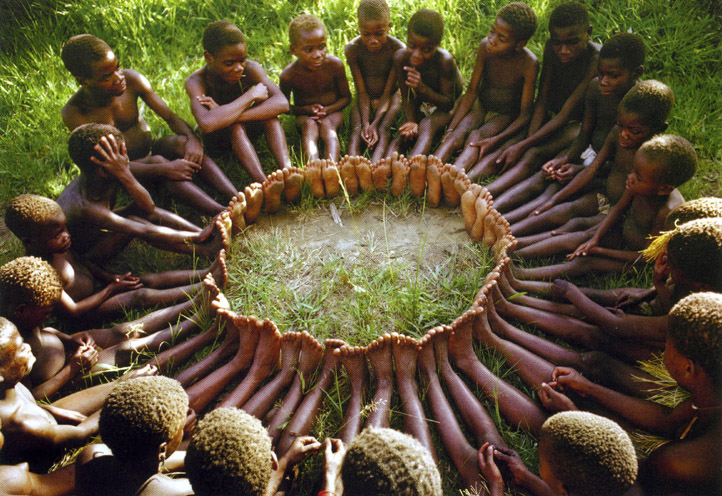
\includegraphics[scale=0.5]{hsubuntuarewe2.jpg}
  \end{center}

\end{frame}

\begin{frame}
  \frametitle{Dúvidas?}
  \begin{itemize}
    \item Os slides estão disponíveis em \url{www.linux.ime.usp.br/\textasciitilde rulojuka/mac0470/pnt.pdf} e serão disponibilizados no paca.\\
    \item O código fonte está disponível em \url{https://github.com/rulojuka/listas}
  \end{itemize}
\end{frame}

\begin{frame}
  \frametitle{Referências}
  \small
  Prólogo:\\
  \vspace{2mm}
  \url{http://en.wikipedia.org/wiki/Timeline_of_historic_inventions}
  \url{http://en.wikipedia.org/wiki/Timeline_of_mathematics}\\
  \vspace{2mm}

  Histórico:\\
  \vspace{2mm}
  \url{http://en.wikipedia.org/wiki/Copyright}
  \url{http://en.wikipedia.org/wiki/History_of_copyright_law}
  \url{http://en.wikipedia.org/wiki/Statute_of_Anne}
  \url{http://en.wikipedia.org/wiki/Berne_Convention}\\
  \vspace{2mm}

  Software Livre:\\
  \vspace{2mm}
  \url{https://www.gnu.org/philosophy/free-sw.pt-br.html}

\end{frame}
\begin{frame}

  Software Livre e Educação:\\
  \vspace{2mm}
  {\footnotesize CPEU3 - Education and Free Software: Jon Maddog Hall:} \href{https://www.youtube.com/watch?v=SOxB1IaozCA}{Vídeo}/\href{https://www.cs.helsinki.fi/linux15vuotta/hall.pdf}{Slides}\\
  \url{http://www.stevehargadon.com/2006/09/interviews-with-maddog-hal_115947326109961843.html}\\
  \href{https://www.youtube.com/watch?v=pfty3d4NnEw}{Free Software And Education}\\
  \href{http://www.technologyreview.com/news/506466/given-tablets-but-no-teachers-ethiopian-children-teach-themselves/}{Given Tablets but No Teachers}\\
  \href{https://www.youtube.com/watch?v=gTKIGo151MQ}{Software livre na educação}\\
  Imagem retirada de \url{http://www.harisingh.com/AllForOneWonForAll.htm}, todos os direitos reservados. :(
\end{frame}
\end{document}